\chapter{Principal Component Analysis \& Statistical Shape \& Appearance Modelling}\label{PCA_CHAP}


\section{Introduction}

\subsection{Aims of Statistical Shape \& Appearance Models}

\subsection{General Methodology}

Generally SSAMs start with a rigid registration, where rotations and translations are applied to all meshes or models that form the input data set so that they share a common coordinate system.
Methods of performing the rigid registration often use an automated approach where certain degrees of freedom are restricted to ensure registration is achieved.



\section{Methods}

\subsection{Measuring Vertebral Geometry}

Vertebral volume or the vertebral body volume may be the easiest and most obvious measure of geometric change within a set of vertebra.
It has been shown in Chapter \ref{Chapter_HT} that there is a strong correlation between vertebral size and stiffness and so this may be enough for a range of comparisons between spines and individual vertebrae.
However, the input set of vertebrae contain a wide range of variation which can be seen visually, which may play an important role in the effect of cement augmentation and is another method of validating the outputs from the PCA generated set of models.

Measuring vertebral geometries in previous studies have either taken the measurements from x-ray scans \cite{Gilad1986,Gilad1985} or $\mu$CT scans \cite{Zhou2000,Cheung1994}, where the measurements have been made through the moving a cursor to the locations of specific points and reporting the distance between them.
While this method may produce accurate results, there is inherent human error associated, the number of measurements is limited to the number of planes available and applying this to large sets of data is time consuming which may lead to further error.

The approach used here involves using the 1 mm voxel resolution models generated in ScanIP (v. 2016) which are are used for FE modelling.
The mask describing the vertebral body of these vertebrae is exported as a stereolithography file (STL), allowing the surface of the vertebra to be measured.
Measuring the vertebra was carried out in Matlab where the STL file was imported forming a point cloud describing the surface from the surface nodes.
Once imported the point cloud was split into thirds in each of the three anatomical planes, with the points describing the vertebra within these thirds being stored in nine array variables.
Cuboids were then fitted to the 3D arrays, maintaining the correct alignment and therefore prohibiting rotation of the cuboid.
The cuboid fits can be seen in \cref{fig:cuboid_ax, fig:cuboid_sag, fig:cuboid_cor}.


\begin{figure}[ht!]
  \centering
  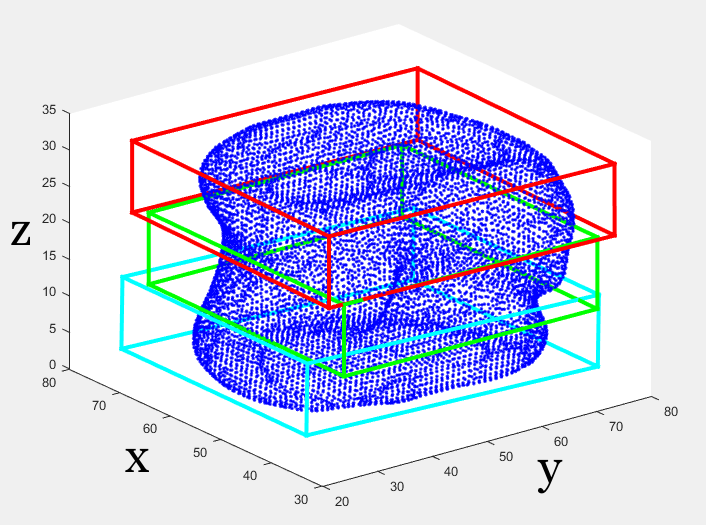
\includegraphics[width=4in]{Chapters/Chapter_PCA_images/Cuboid_fit_axial.png}
  \caption{The three cuboids fitted to the vertebra point cloud in the axial plane.}
  \label{fig:cuboid_ax}
\end{figure}

\begin{figure}[ht!]
  \centering
  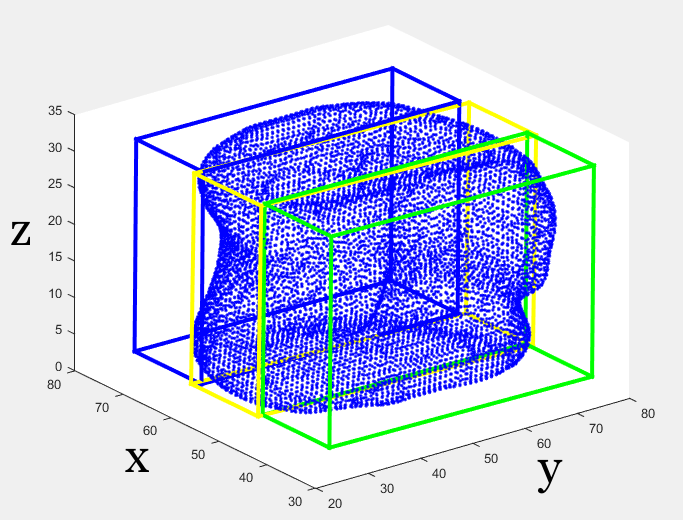
\includegraphics[width=4in]{Chapters/Chapter_PCA_images/Cuboid_fit_coronal.png}
  \caption{The three cuboids fitted to the vertebra point cloud in the coronal plane.}
  \label{fig:cuboid_cor}
\end{figure}

\begin{figure}[ht!]
  \centering
  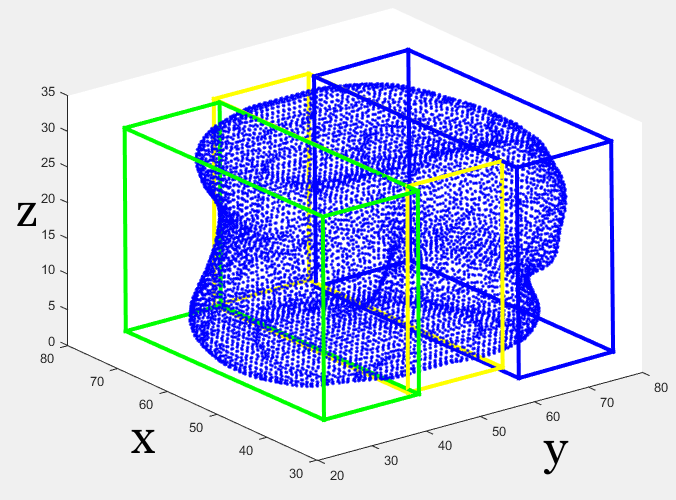
\includegraphics[width=4in]{Chapters/Chapter_PCA_images/Cuboid_fit_sagital.png}
  \caption{The three cuboids fitted to the vertebra point cloud in the sagital plane.}
  \label{fig:cuboid_sag}
\end{figure}

Measuring the two longer sides of the fitted cuboids gives a total of 18 measurements describing most aspects of the vertebral geometry, these can be seen with their abbreviations in Table \ref{tab:measurements}.
This includes identifying wedge shaped vertebrae, recorded as reduced anterior height compared to the posterior height, left to right wedge shapes, recorded as sagital left height being smaller or larger when compared to the sagital right height.

\begin{table}[ht!]
	\caption{The measurements and abbreviations taken from the vertebrae.}
	\label{tab:measurements}
	\centering
	\begin{tabular}{c|c}
    Measurement & Abbreviation \\
    \hline
    \hline
    Sagital Left Height & SLH \\
	Sagital Left Depth & SLD \\
    Sagital Mid Height & SMH \\
	Sagital Mid Depth & SMD \\
    Sagital Right Height & SRH \\
	Sagital Right Depth & SRD \\
	Coronal Anterior Height & CAH \\
	Coronal Anterior Width & CAW \\
	Coronal Mid Height & CMH \\
	Coronal Mid Width & CMW \\
	Coronal Posterior Height & CPH \\
	Coronal Posterior Width & CPW \\
	Axial Inferior Depth & AID \\
	Axial Inferior Width & AIW \\
	Axial Mid Depth & AMD \\
	Axial Mid Width & AMW \\
	Axial Superior Depth & ASD \\
	Axial Superior Width & ASW \\
	\hline
	\end{tabular}
\end{table}

The plugin for ScanIP that allows principal component analysis and the generation of models described by the principal components consists of five main steps.

The first of these steps is a pre-processing step, converting the masks and backgrounds into nessessary formats (.mha \& .mhd) for use with the ITK toolkit.

The following step carries out rigid registration of the models, aligning the masks and backgrounds to a shared coordinate system.
This is carried out using the ITK library with the registration being measured according to a mean squared image-to-image metric using a gradient descent optimiser.
A limit to the number of attempts or steps allowed can be set; the default value of 100 steps for each input model was used.

The geometry of each input specimen was described in a deformable registration step, measuring the transform required to morph the mean of the input vertebrae onto each of the input vertebrae.
This step utilises the ITK FEM registration filter.

Penultimately, the transforms between the mean and each of the input vertebrae which describe the vertebral geometries are used as inputs for PCA.
Here the outputs of the step include the principal components, their eigenvalue, percentage of variation captured in that component and the cumulative percentage variation captured.

Finally, the SSAM produced can be used with the ITK Image Warp filter to generate new mask and background combinations from within the envelope of geometric and material property variation created by the input set, according to the principal components.
The plugin allows for the first five principal components (PC1, PC2, PC3, PC4 \& PC5) to be used for as variables for model generation, altering the value of the principal components by up to three standard deviations away from the mean in both positive and negative directions.

\subsection{Generating Vertebrae Models}

\subsubsection{Range of Shapes Generated}

To attempt to understand what each of the principal components represented in terms of the variation captured by it, models were created at $\pm$1, $\pm$2 and $\pm$3 standard deviations away from the mean for the first three principal components independently.
In addition to these, the mean model was generated, allowing comparisons of the other generated models against it.

Finally, in order to know whether the range of geometries, material properties and resultant stiffnesses found in the input set was represented in the SSAM within the first three principal components, models were generated which incorporated the variation found in PC1, PC2 \& PC3.
These models would represent the corners of a cube who's axis would be PC1, 2 \& 3 and who's origin would be the mean vertebra.
If the majority of input models (68 \%, representing the quantity of the population expected to fit within $\pm$1 SD of the mean for a normally distributed input set) fit within the limits created by a cube with side length from +1 to -1 SD along each axis for geometric measurements, greyscale background and resultant stiffness, then the variation of the input set will have been captured and represented by the SSAM.

\subsubsection{FE Model Setup}

Once the vertebrae were generated using the plugin the rest of the FE model was set up.
This included forming endcaps to mimic the experimental setup and how the input set was loaded.
Endcaps were created programmaticaly within the ScanIP python scripting environment with a diameter of 90 mm, approximately equal to the diameter of the experimental endcaps, with a depth of 6 mm ensuring the superior and inferior tips of the vertebrae were captured with a minimum of 1 mm between the vertebra and end of the cement.
The remaining properties for the FE model are identical to those used for the models of the human vertebra which became the inputs to the PCA plugin.
This includes a tied interaction between the vertebrae and endcaps and material properties for the endcaps being: Young's modulus 2.45 GPa and Poissons's ratio of 0.3.
Material properties for the vertebra used the same greyscale approach as in previous chapters with the Young's modulus for each element being:
\[ E = GS \times \alpha \]
Where, $GS$ is the greyscale value for the current element (between 0 and 255) and $\alpha$ is the conversion factor.
The conversion factor used has the same value used previously for the non-augmented set of vertebrae: $\alpha = 0.0008184$.
Applying load to the models is carried out as in the previous chapter, with 1 mm of displacement applied to a loading point, with the reaction force being measured to obtain the stiffness.
The loading point is found by finding the centre of the vertebral body in the middle slice axially and translating the point axially to the maximum height of the model, including endcaps.
The load is then applied through a plate which is tied to the superior endcap.

\subsubsection{Augmentation in Generated Models}




\section{Results}
\subsection{Measuring \& Interrogating Vertebral Variation}

\subsubsection{Geometry Variation}

The geometric variation found in the first three principal components has been identified using the images of the surface point clouds of the mean and +3 and -3 standard deviations away from the mean, along with the measurements of the 18 variables described previously.
The images of the point clouds can be seen in \cref{fig:PC1_2_3_Axial,fig:PC1_2_3_Sagital,fig:PC1_2_3_Coronal}, showing the view of the vertebral models from the three anatomical planes with a three-dimensional view in \cref{fig:PC1_2_3_3D}.
More simplified figures can be seen in \cref{fig:PC1_2_3_AxialSlice,fig:PC1_2_3_SagitalSlice,fig:PC1_2_3_CoronalSlice}, showing the mid-slice through each of the anatomical planes, while information is lost here, it allows an clear visualisation of the modes of variation found in the main parts of the vertebral body.
Here, only the +3, mean and -3 standard deviations of the principal components are shown, this simplifies and allows clear visualisations of the main mode of variation present in each principal component.
A quantification of the change in volume can be seen in \cref{tab:pca_geo_tab} for the mean and $\pm$ 1, 2 \& 3 standard deviations away from the mean.

Principal component one contains the least geometric variation of the first three principal components.
The mid slice axially shows an almost identical shape and size between the +3, mean and -3 standard deviations, while the coronal and sagittal planes show minor changes in the overall size and volume of the vertebrae.
The changes in total vertebral volume is limited to 17 \% larger and 15 \% smaller than the mean model, shown in \cref{tab:pca_geo_tab}.

Principal component two shows the most interesting geometric variation with many of the different shapes and some of the degeneration of the input set clearly visible.
The large changes to the axial mid slice (\cref{fig:PC1_2_3_AxialSlice}) of the second principal component appear to represent the different levels of the lumbar spine that made up the input set.
Positive standard deviations away from the mean, especially the +3 SD slice has the much wider posterior portion aligning with that of the L5 lumbar vertebrae.
Conversely the much narrower -3 SD model appears similar to the L1 lumbar vertebrae.
This change in width between the +3 and -3 SD is especially evident in the coronal views in \cref{fig:PC1_2_3_CoronalSlice}.
This change from vertebra reminiscent of L5 vertebrae at +3 SD to L1 vertebra at -3 SD (and therefore L3 vertebrae in the mean model) is also reflected in the sagittal views (\cref{fig:PC1_2_3_SagitalSlice}) where anterior and posterior wedge shapes can be seen in the +3 and -3 SD models respectively.

Finally, principal component three also contains a considerable quantity of the geometric variation, although much more simple.
Here, the mode of geometric variation is the size of the vertebrae with the -3 SD model being considerably larger than the mean vertebral model (54 \% larger) and vice versa with the +3 SD model, where its volume is much smaller than the mean vertebra (40 \% smaller).

Quantification of all of the measurements taken on the generated models can be seen in \cref{tab:pca_geo_tab} with the acronyms for the measurements given in \cref{tab:measurements}.
The colouration in the table allows easy identification of the changes to the vertebral geometry compared to the mean generated model, for example, while the changes to the measurements are near uniform in PC 1 \& 3, the non-uniform nature of PC 2 shows the different shapes that are present and described above.
Additionally it allows quantification of the shapes seen in the models, for example the anterior and posterior wedge shapes in PC 2, described with the Coronal Anterior Height and the Coronal Posterior Height having an antagonistic relationship.
However, the main benefit of the table and its measurements is for the validation of the PC models against the input set, ensuring that the shapes measured in the input set are represented in the models.
This is described in \cref{sec:pca_val}.


\begin{figure}[p]
  \centering
  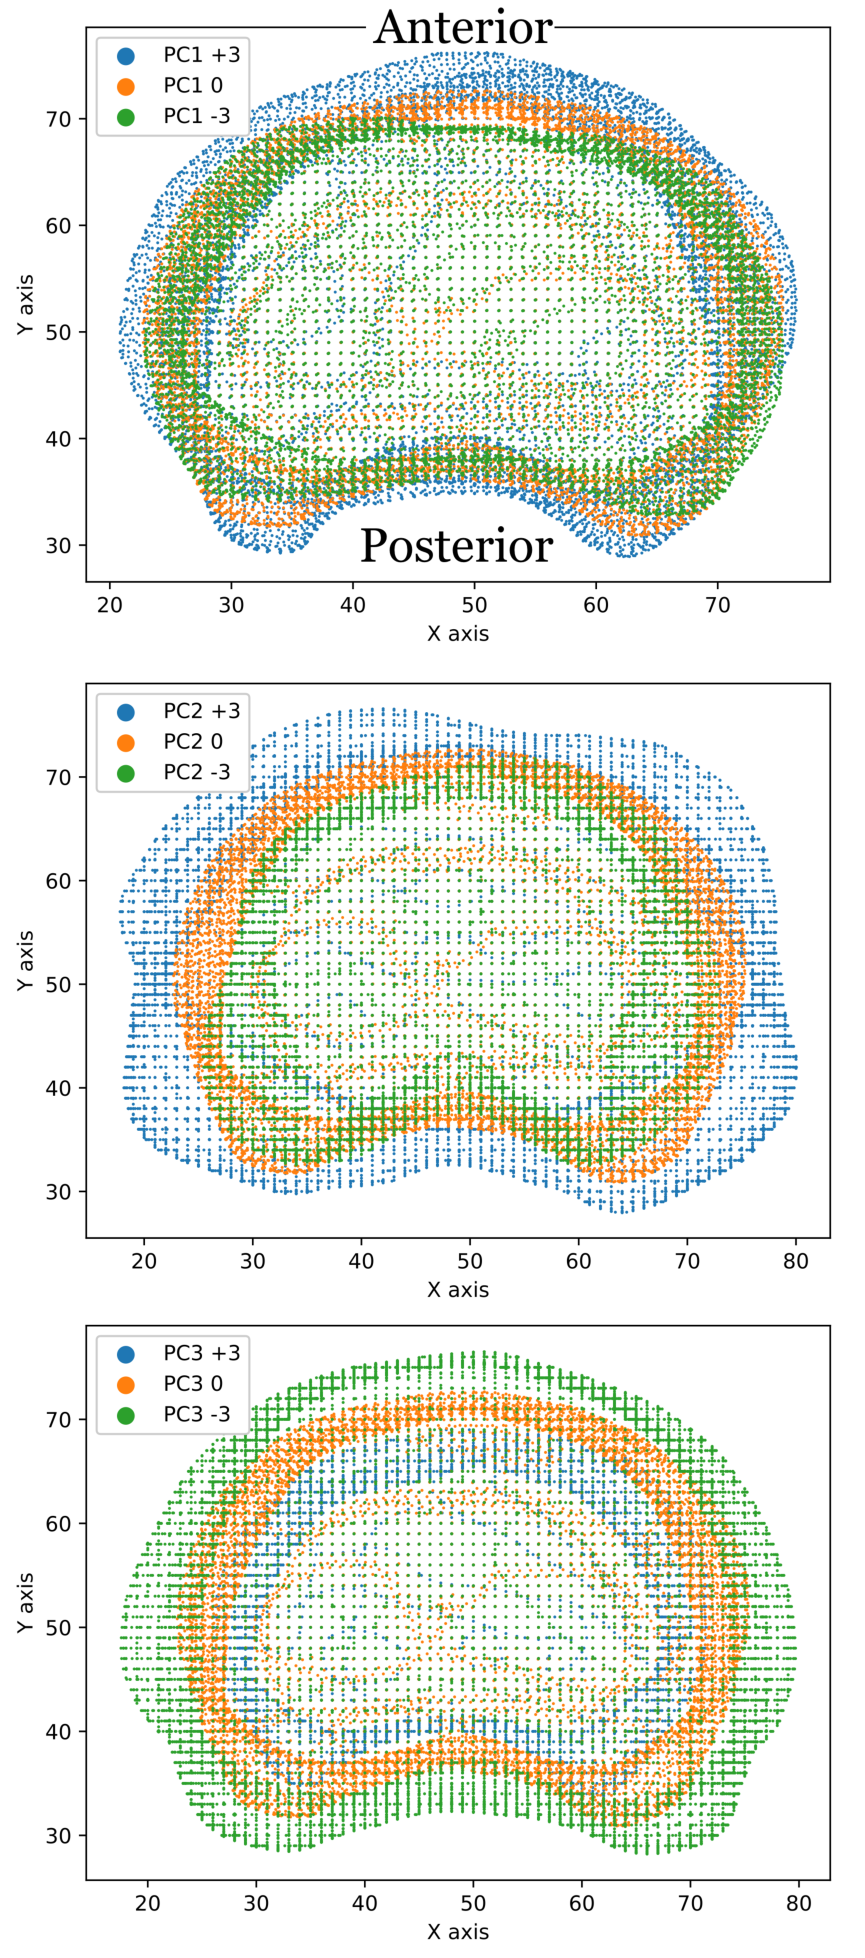
\includegraphics[width=.65\textwidth]{Chapters/Chapter_PCA_images/PC1_2_3_Axial.pdf}
  \caption{Axial views of the surface point clouds of the vertebral models from the first three principal components, showing the mean, +3 and -3 standard deviations away from the mean. Showing how the geometry is captured in the first three principal components.}
  \label{fig:PC1_2_3_Axial}
\end{figure}

\begin{figure}[p]
  \centering
  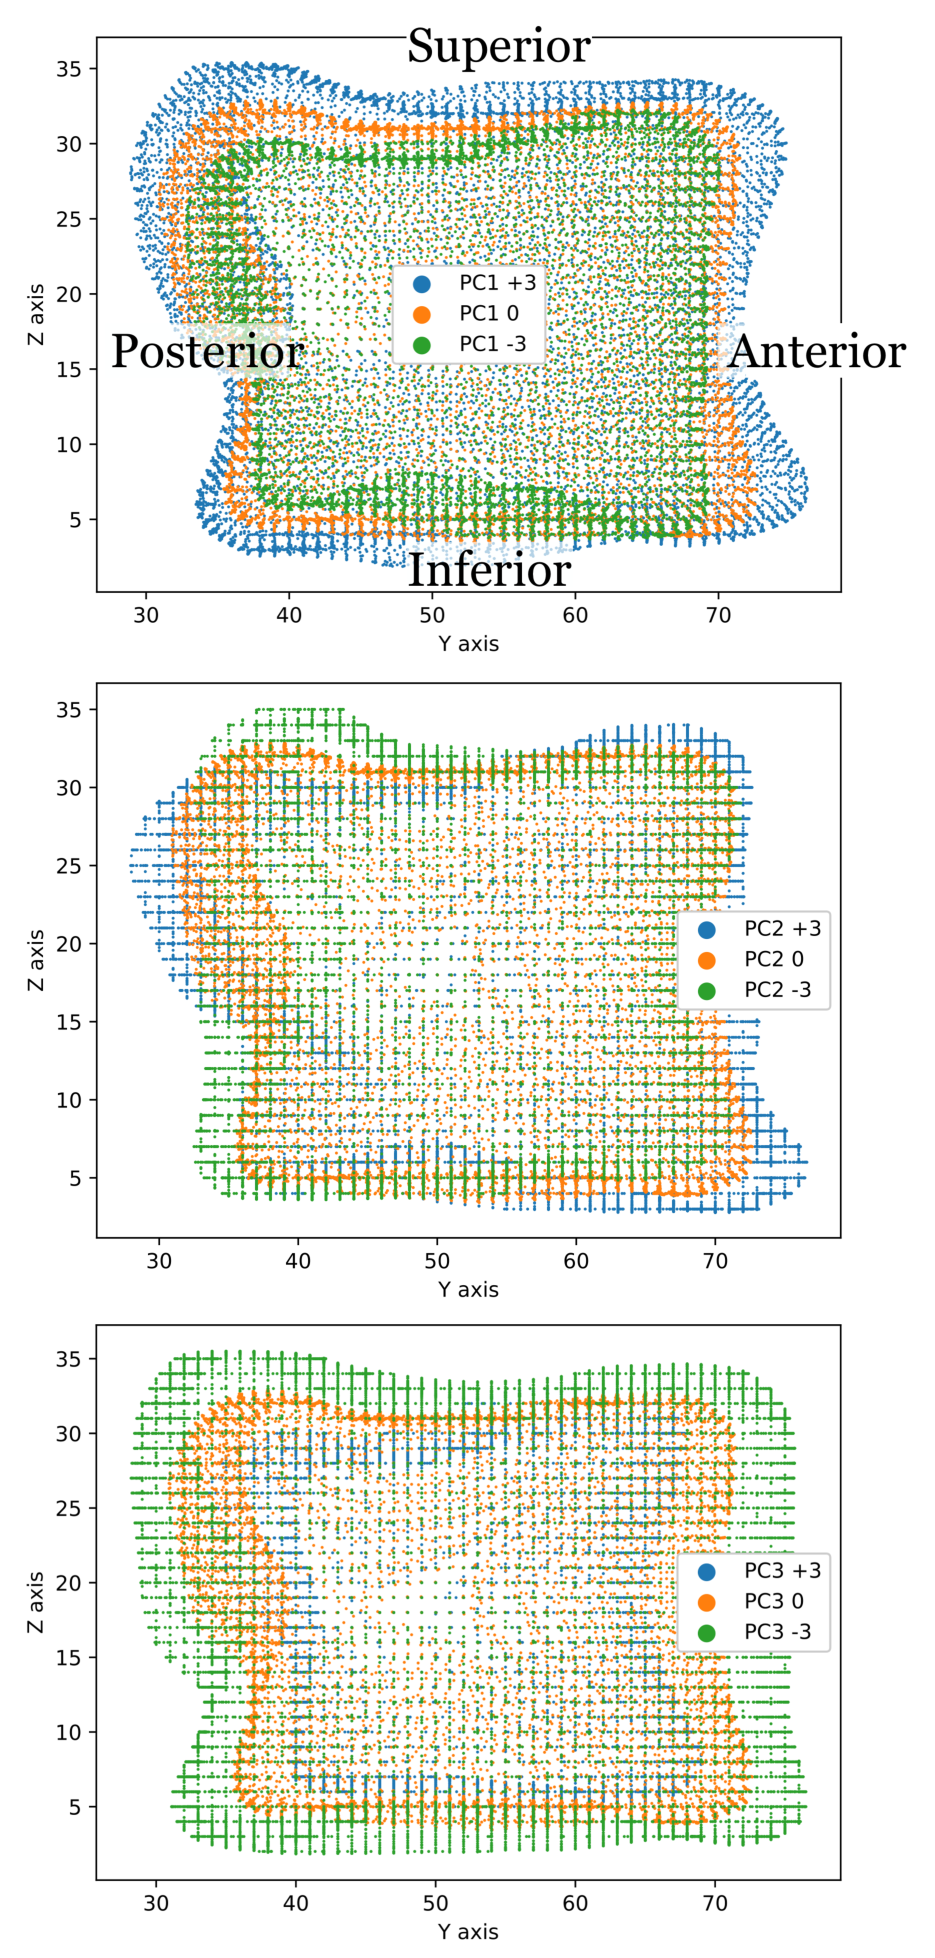
\includegraphics[width=.65\textwidth]{Chapters/Chapter_PCA_images/PC1_2_3_Sagital.pdf}
  \caption{Sagittal views of the surface point clouds of the vertebral models from the first three principal components, showing the mean, +3 and -3 standard deviations away from the mean. Showing how the geometry is captured in the first three principal components.}
  \label{fig:PC1_2_3_Sagital}
\end{figure}

\begin{figure}[p]
  \centering
  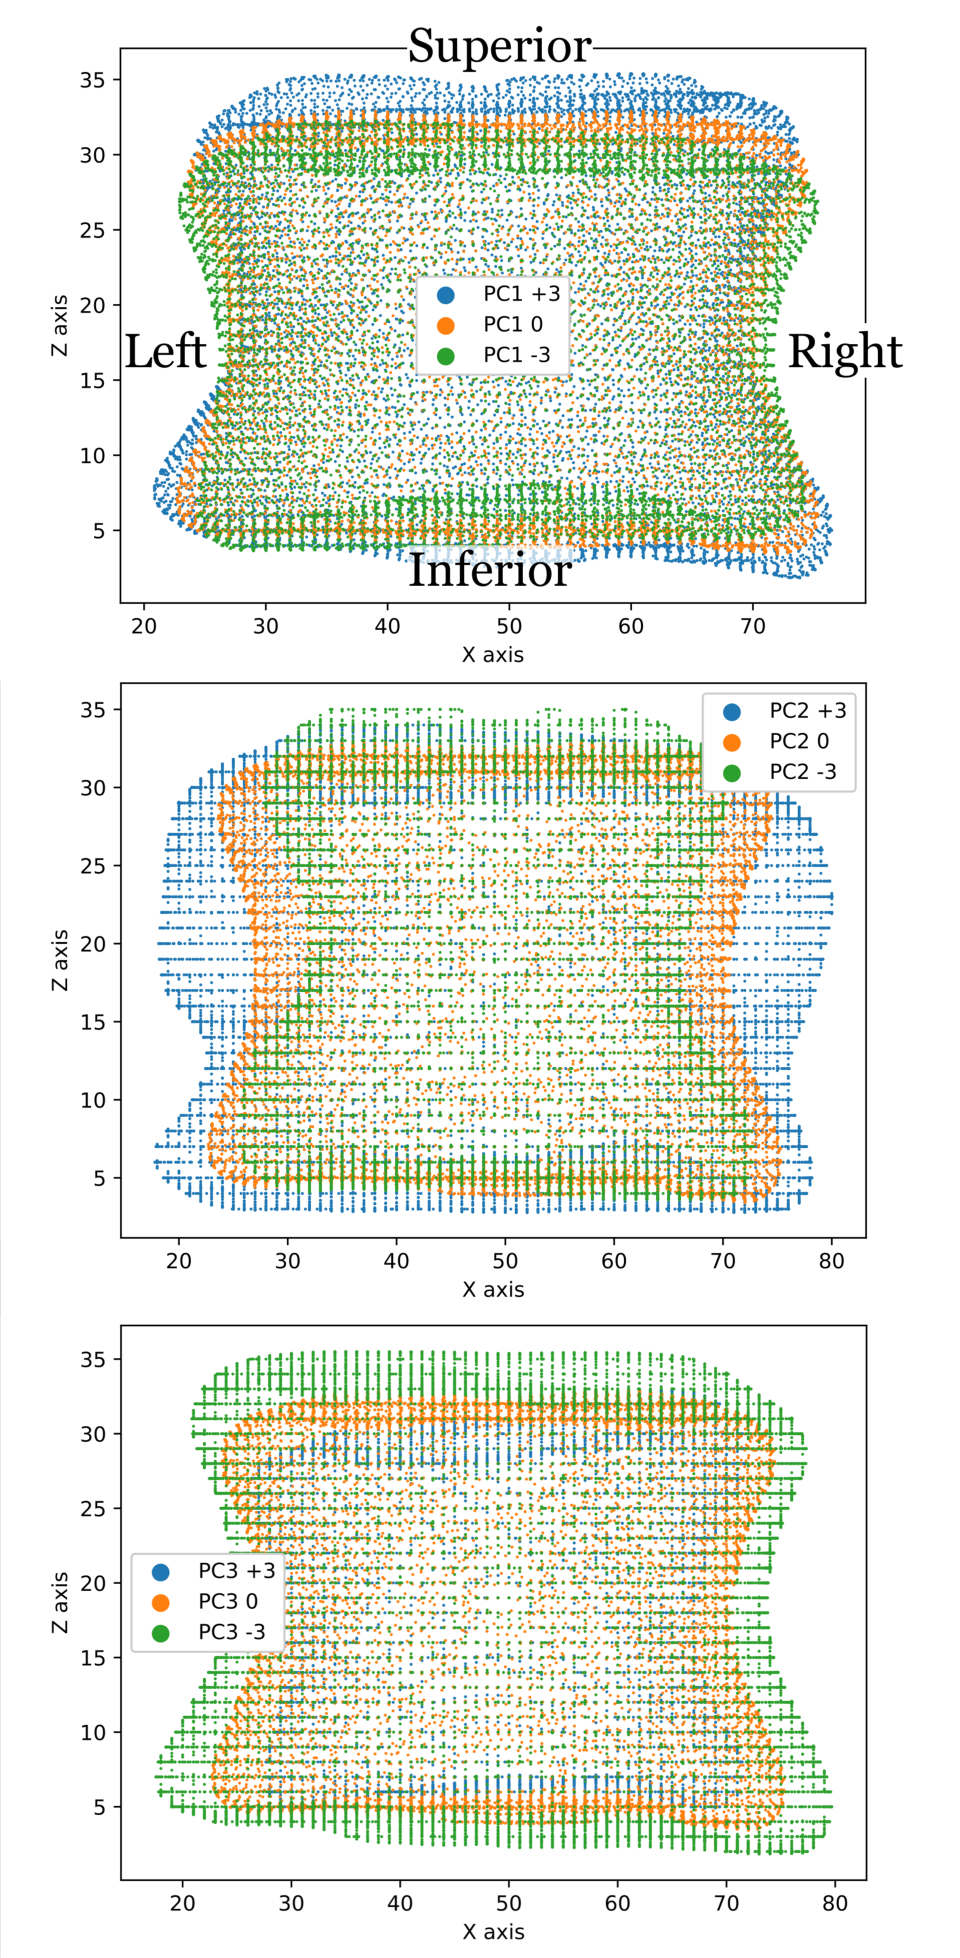
\includegraphics[width=.65\textwidth]{Chapters/Chapter_PCA_images/PC1_2_3_Coronal.pdf}
  \caption{Coronal views of the surface point clouds of the vertebral models from the first three principal components, showing the mean, +3 and -3 standard deviations away from the mean. Showing how the geometry is captured in the first three principal components.}
  \label{fig:PC1_2_3_Coronal}
\end{figure}



\begin{figure}[p]
  \centering
  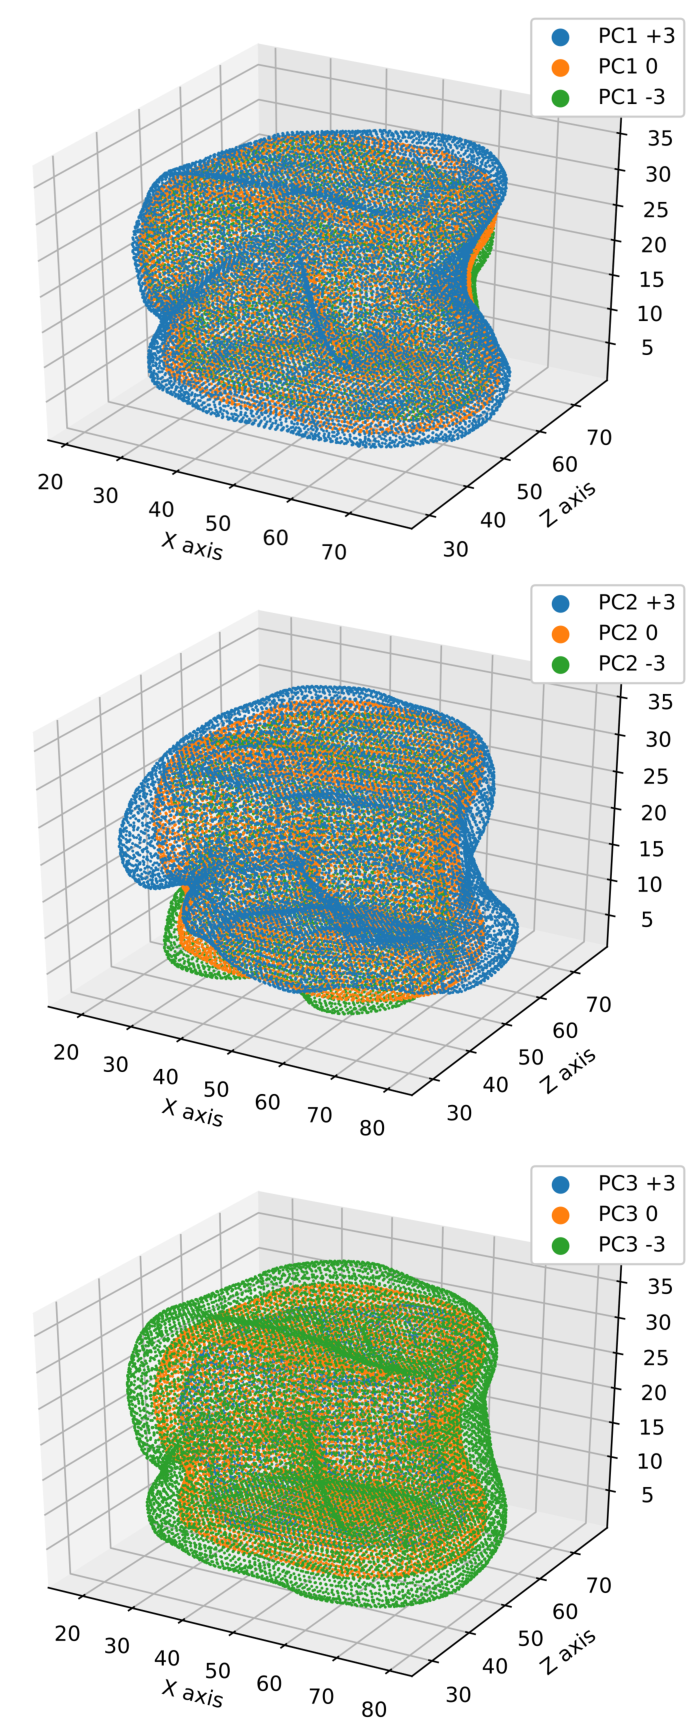
\includegraphics[width=.65\textwidth]{Chapters/Chapter_PCA_images/PC1_2_3_3D.pdf}
  \caption{Three dimensional views of the surface point clouds of the vertebral models from the first three principal components, showing the mean, +3 and -3 standard deviations away from the mean. Showing how the geometry is captured in the first three principal components.}
  \label{fig:PC1_2_3_3D}
\end{figure}


\begin{figure}[p]
  \centering
  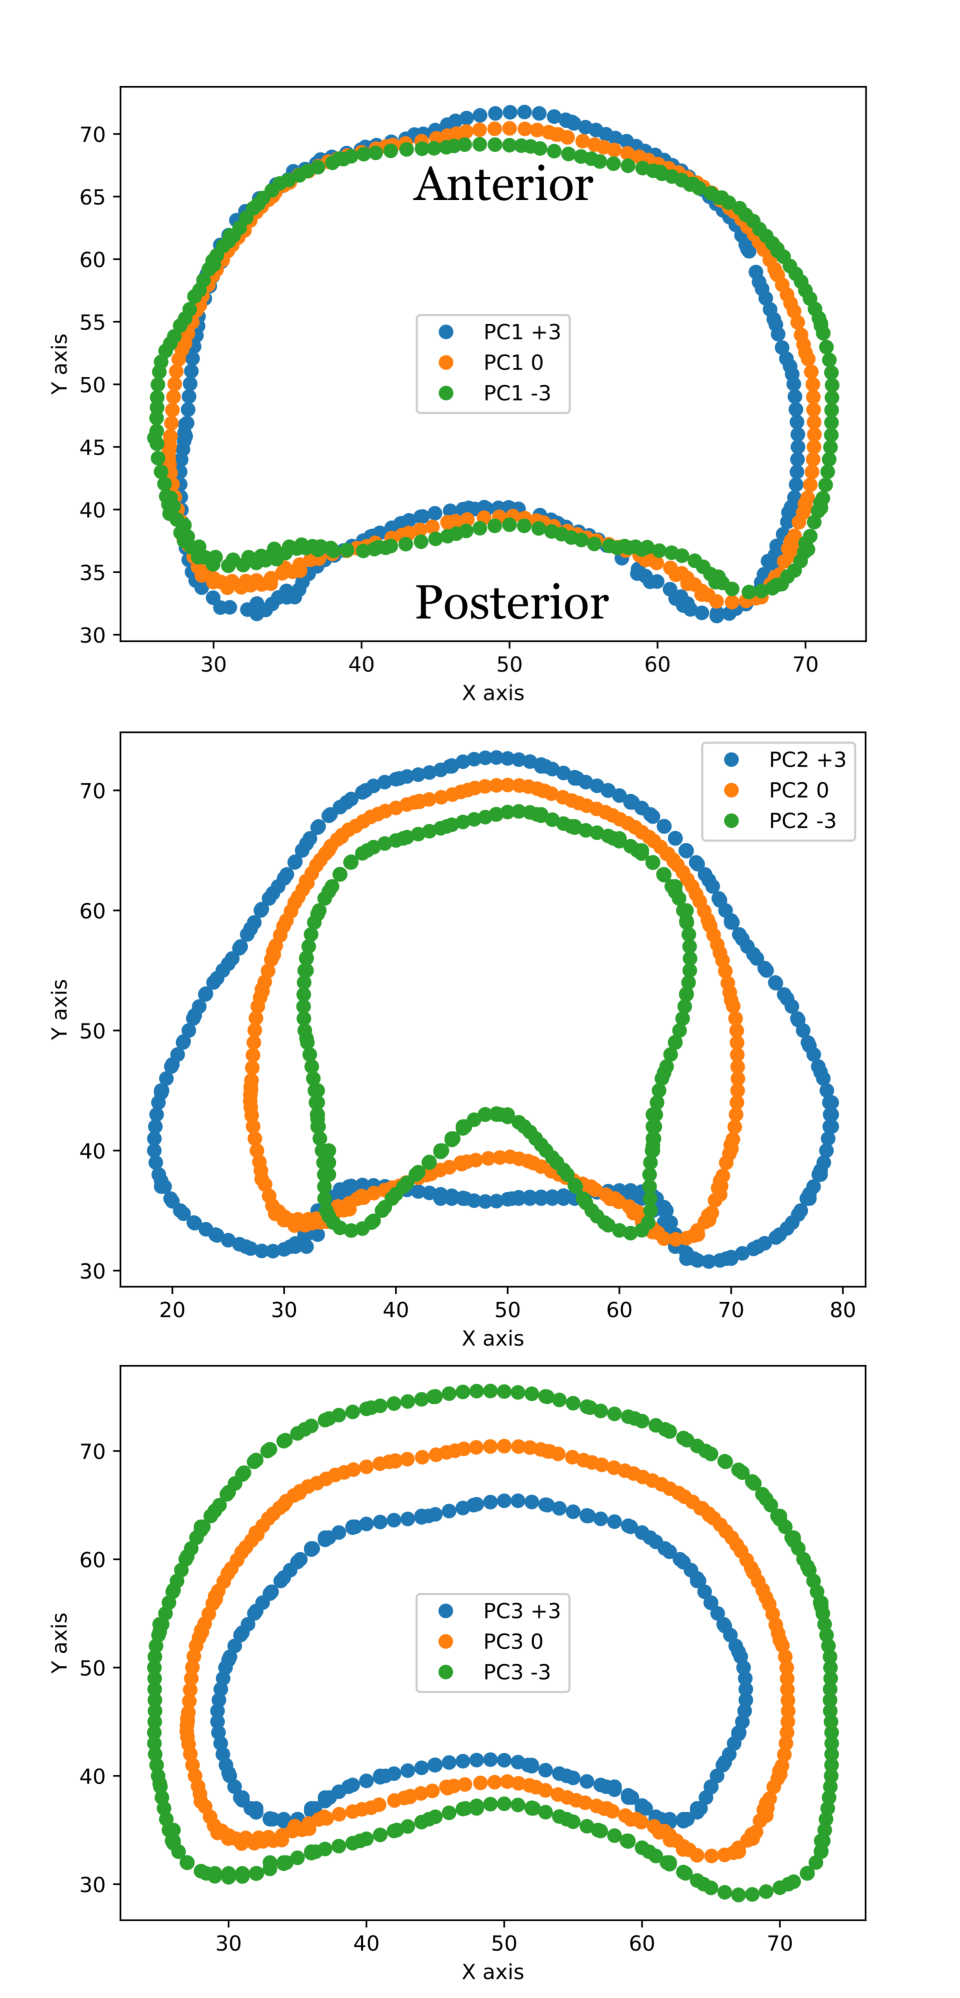
\includegraphics[width=.65\textwidth]{Chapters/Chapter_PCA_images/PC1_2_3_AxialSlice.pdf}
  \caption{Axial views of the mid slice of the vertebral models from the first three principal components, showing the mean, +3 and -3 standard deviations away from the mean. Showing how the geometry is captured in the first three principal components.}
  \label{fig:PC1_2_3_AxialSlice}
\end{figure}

\begin{figure}[p]
  \centering
  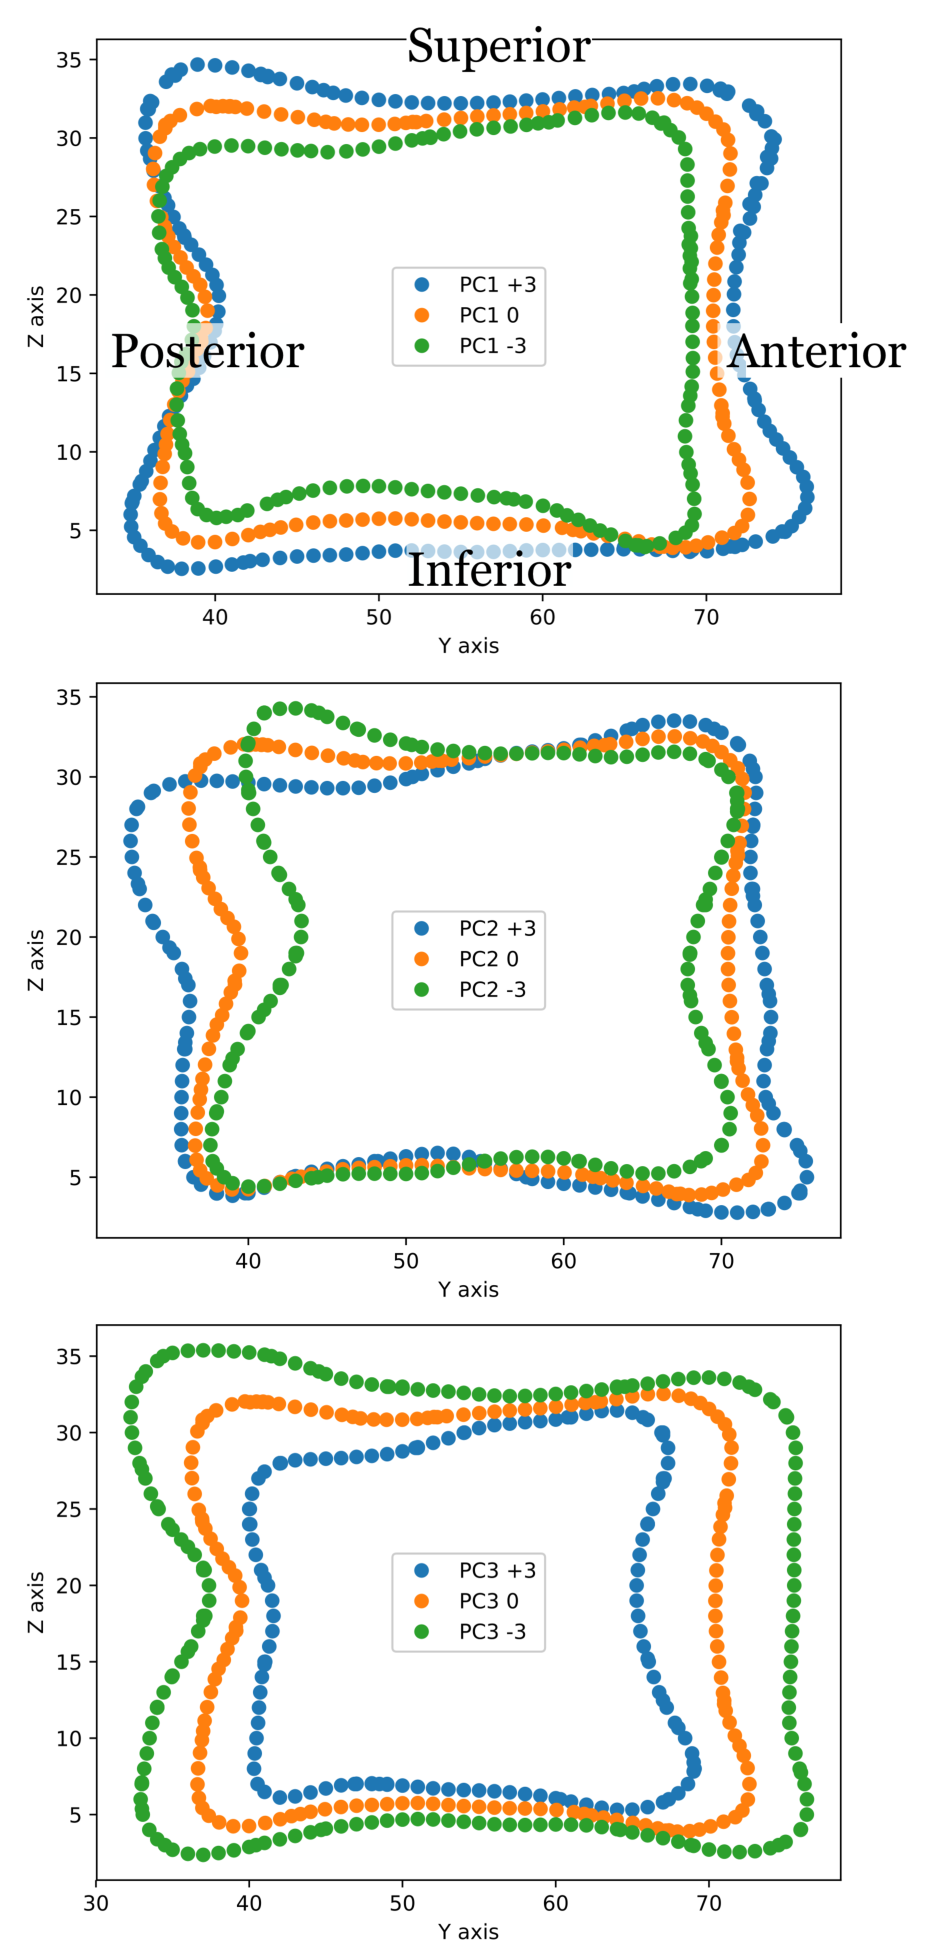
\includegraphics[width=.65\textwidth]{Chapters/Chapter_PCA_images/PC1_2_3_SagitalSlice.pdf}
  \caption{Sagittal views of the mid slice of the vertebral models from the first three principal components, showing the mean, +3 and -3 standard deviations away from the mean. Showing how the geometry is captured in the first three principal components.}
  \label{fig:PC1_2_3_SagitalSlice}
\end{figure}

\begin{figure}[p]
  \centering
  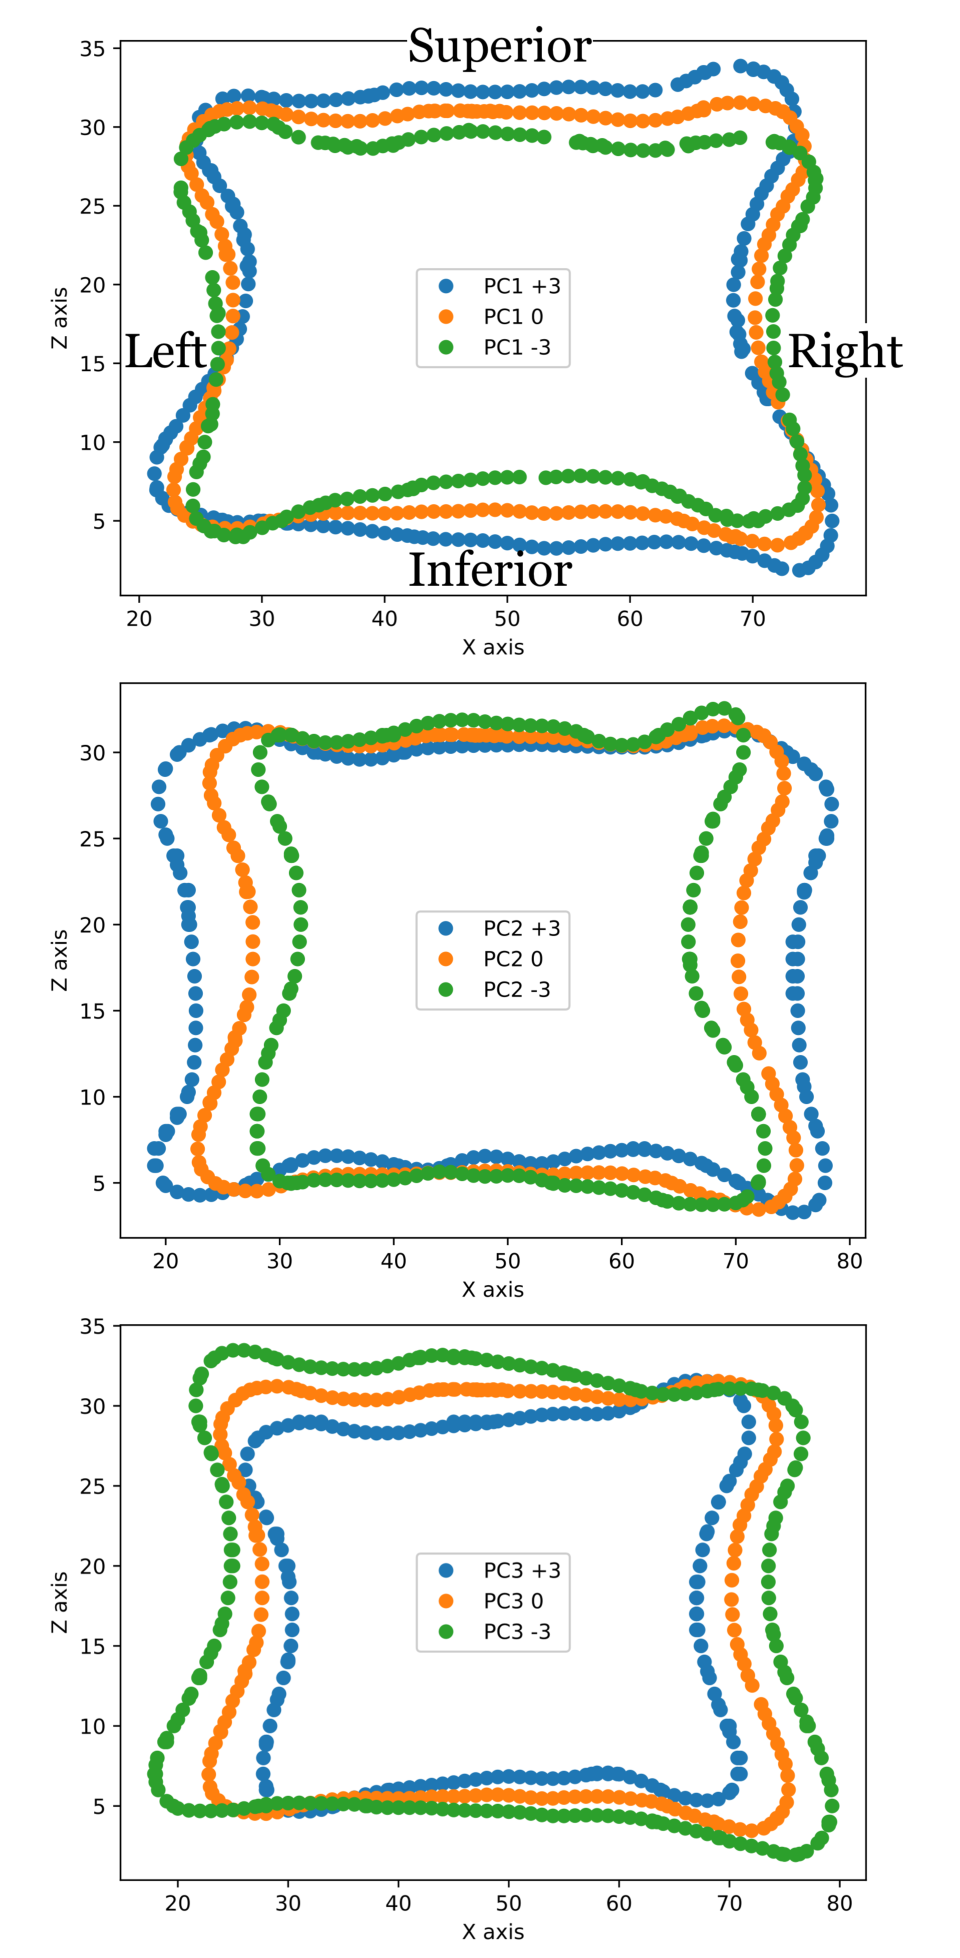
\includegraphics[width=.65\textwidth]{Chapters/Chapter_PCA_images/PC1_2_3_CoronalSlice.pdf}
  \caption{Coronal views of the mid slice of the vertebral models from the first three principal components, showing the mean, +3 and -3 standard deviations away from the mean. Showing how the geometry is captured in the first three principal components.}
  \label{fig:PC1_2_3_CoronalSlice}
\end{figure}

\begin{table}[p]
\centering
\caption{The volume of the principal component models as a fraction of the mean model's volume, showing how much of the volumetric variation is captured in each of the principal components. }
\label{tab:pc_vol}
\begin{tabular}{c|c}
Principal Component & Voxel Count Fraction       \\ \hline \hline
PC1 +3               & 1.171 \\
PC1 +2               & 1.108 \\
PC1 +1               & 1.055 \\
Mean                 & 1.000 \\
PC1 -1               & 0.947 \\
PC1 -2               & 0.897 \\
PC1 -3               & 0.847 \\ \hline

PC2 +3               & 1.228 \\
PC2 +2               & 1.152 \\
PC2 +1               & 1.081 \\
Mean                 & 1.000 \\
PC2 -1               & 0.937 \\
PC2 -2               & 0.869 \\
PC2 -3               & 0.802 \\ \hline

PC3 +3               & 0.600 \\
PC3 +2               & 0.720 \\
PC3 +1               & 0.854 \\
Mean                 & 1.000 \\
PC3 -1               & 1.163 \\
PC3 -2               & 1.344 \\
PC3 -3               & 1.538 \\ \hline
\end{tabular}
\end{table}

\begin{landscape}

\begin{table}[p]
  \centering
  \caption{The measurements of the 18 variables (abbreviations in \cref{tab:measurements}), shown as a fraction of the mean models measurements. Colouration shows the reduced measurements in red and larger measurements in green showing the geometric variation quantitatively.}
  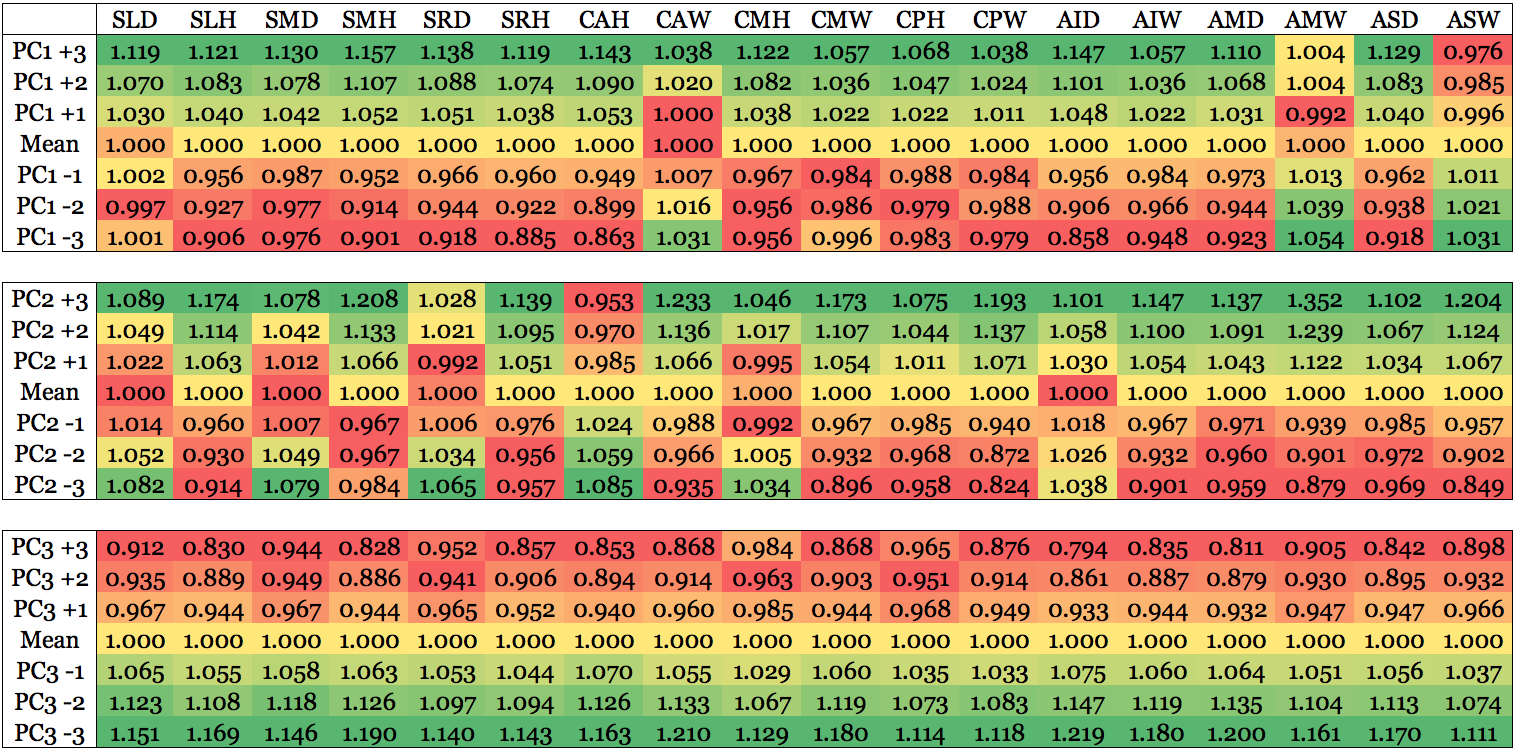
\includegraphics[width=1.7\textwidth]{Chapters/Chapter_PCA_images/pca_geo_table.png}
  \label{tab:pca_geo_tab}
\end{table}

\end{landscape}

\pagebreak



\subsubsection{Greyscale \& Material Property Variation}

\begin{figure}[p]
  \centering
  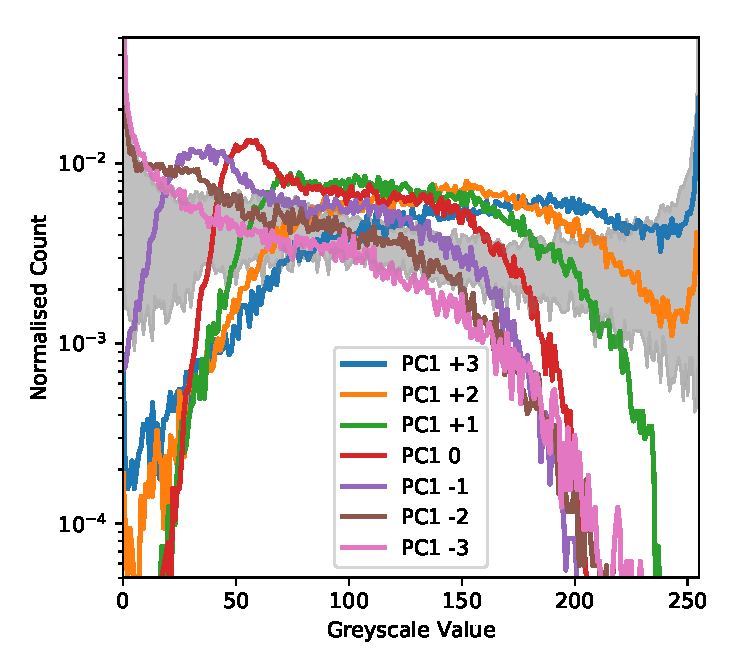
\includegraphics[width=.65\textwidth]{Chapters/Chapter_PCA_images/pca1_histo.pdf}
  \caption{Histogram of the models generated from principal component 1, with $\pm$ 3, 2 \& 1 standard deviations away from the mean. The values are normalised with respect to the total volume of the vertebrae, allowing comparisons with different sized model. The grey background represents the range of histograms seen in the input set.}
  \label{fig:pca1_histo}
\end{figure}

\begin{figure}[p]
  \centering
  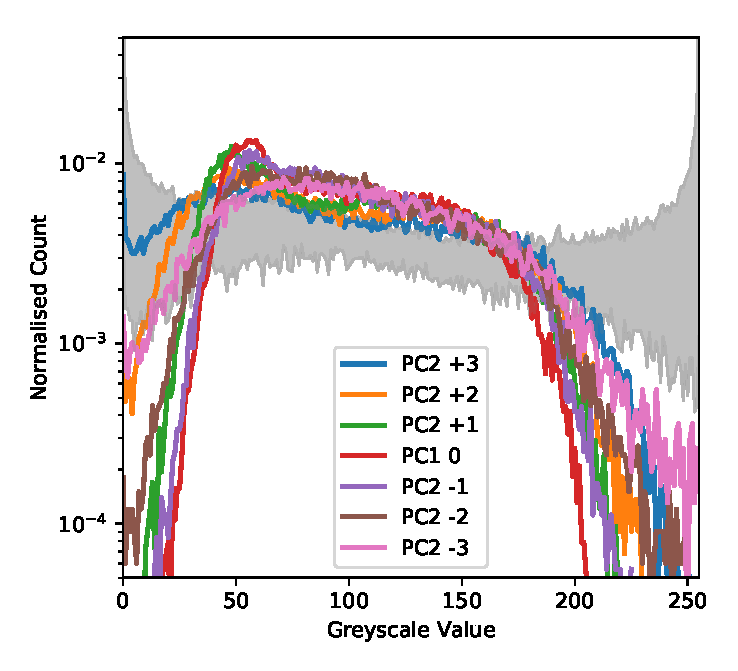
\includegraphics[width=.65\textwidth]{Chapters/Chapter_PCA_images/pca2_histo.pdf}
  \caption{Histogram of the models generated from principal component 2, with $\pm$ 3, 2 \& 1 standard deviations away from the mean. The values are normalised with respect to the total volume of the vertebrae, allowing comparisons with different sized model. The grey background represents the range of histograms seen in the input set.}
  \label{fig:pca2_histo}
\end{figure}

\begin{figure}[p]
  \centering
  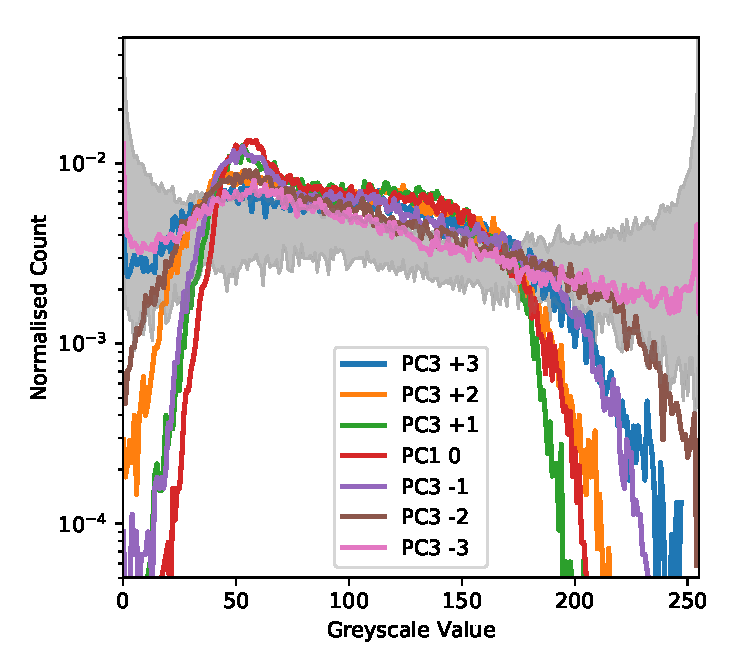
\includegraphics[width=.65\textwidth]{Chapters/Chapter_PCA_images/pca3_histo.pdf}
  \caption{Histogram of the models generated from principal component 3, with $\pm$ 3, 2 \& 1 standard deviations away from the mean. The values are normalised with respect to the total volume of the vertebrae, allowing comparisons with different sized model. The grey background represents the range of histograms seen in the input set.}
  \label{fig:pca3_histo}
\end{figure}

%TODO add image comparing the pca model background and the input model background

\subsubsection{Resulting Stiffness Variation}

\subsection{Validating Generated Vertebrae} \label{sec:pca_val}

Validation of the generated vertebrae from the PCA plugin for scanIP is vital for ensuring any results are sensible, for example when artificially augmenting the vertebrae, and to ensure that the modes of variation previously described are genuine descriptions of the variation found within the input set.
To achieve this validation, aspects important to the generated models need to be compared to the variables found in the input set.
The variables compared will be the geometry and volume of the vertebrae, the greyscale background and therefore the material properties of the models and finally the resulting stiffness when loads are simulated on the generated FE model.
While identifying the modes of variation in isolation are important to characterise how such variation affects the outcomes of augmentation or understanding the content and main modes of variation, combinations of the principal components generate different models that may describe different ranges of variation.
Therefore, the variation found within one standard deviation of the mean for the first three principal components, including all of the combinations of standard deviations within $\pm$ 1 SD, including the mean.
For example, PC 1 +1, PC 2 +1, PC 3 -1, would be one model with a combination of the first three principal components.

\subsubsection{Geometry Validation}

Identifying the variation in geometry for combinations of the first three principal components, with all possible combinations within $\pm$1 SD of the mean is presented here.
The 18 geometric measures found within the $\pm$1 SD models are presented in \cref{fig:pca_cube}. 
The results presented here show a strong agreement between the input and the generated models, with the means of the two sets agreeing closely, along with the range of the measurements.
Outliers in the input set originate from the bone spurs and other features of the degenerated vertebrae. %TODO add image of G19 L1
Differences in the range of generated vertebrae compared to the range of measurements seen in the input set are due to the input set describing only one standard deviation of variation.

Volume differences between the input set and generated vertebrae were also small, with the difference between the mean of the input set volume and the mean generated model volume being 10 \%, the means being 39500 mm$^3$ and 38245 mm$^3$ respectively.
The range of vertebral volumes is also comparable: the input set range is 31189 to 56003 mm$^3$ while the generated vertebrae for $\pm$1 SD with all possible combinations of PC 1, 2 and 3, have a range of 28152 to 50462 mm$^3$.

\begin{figure}[h]
  \centering
  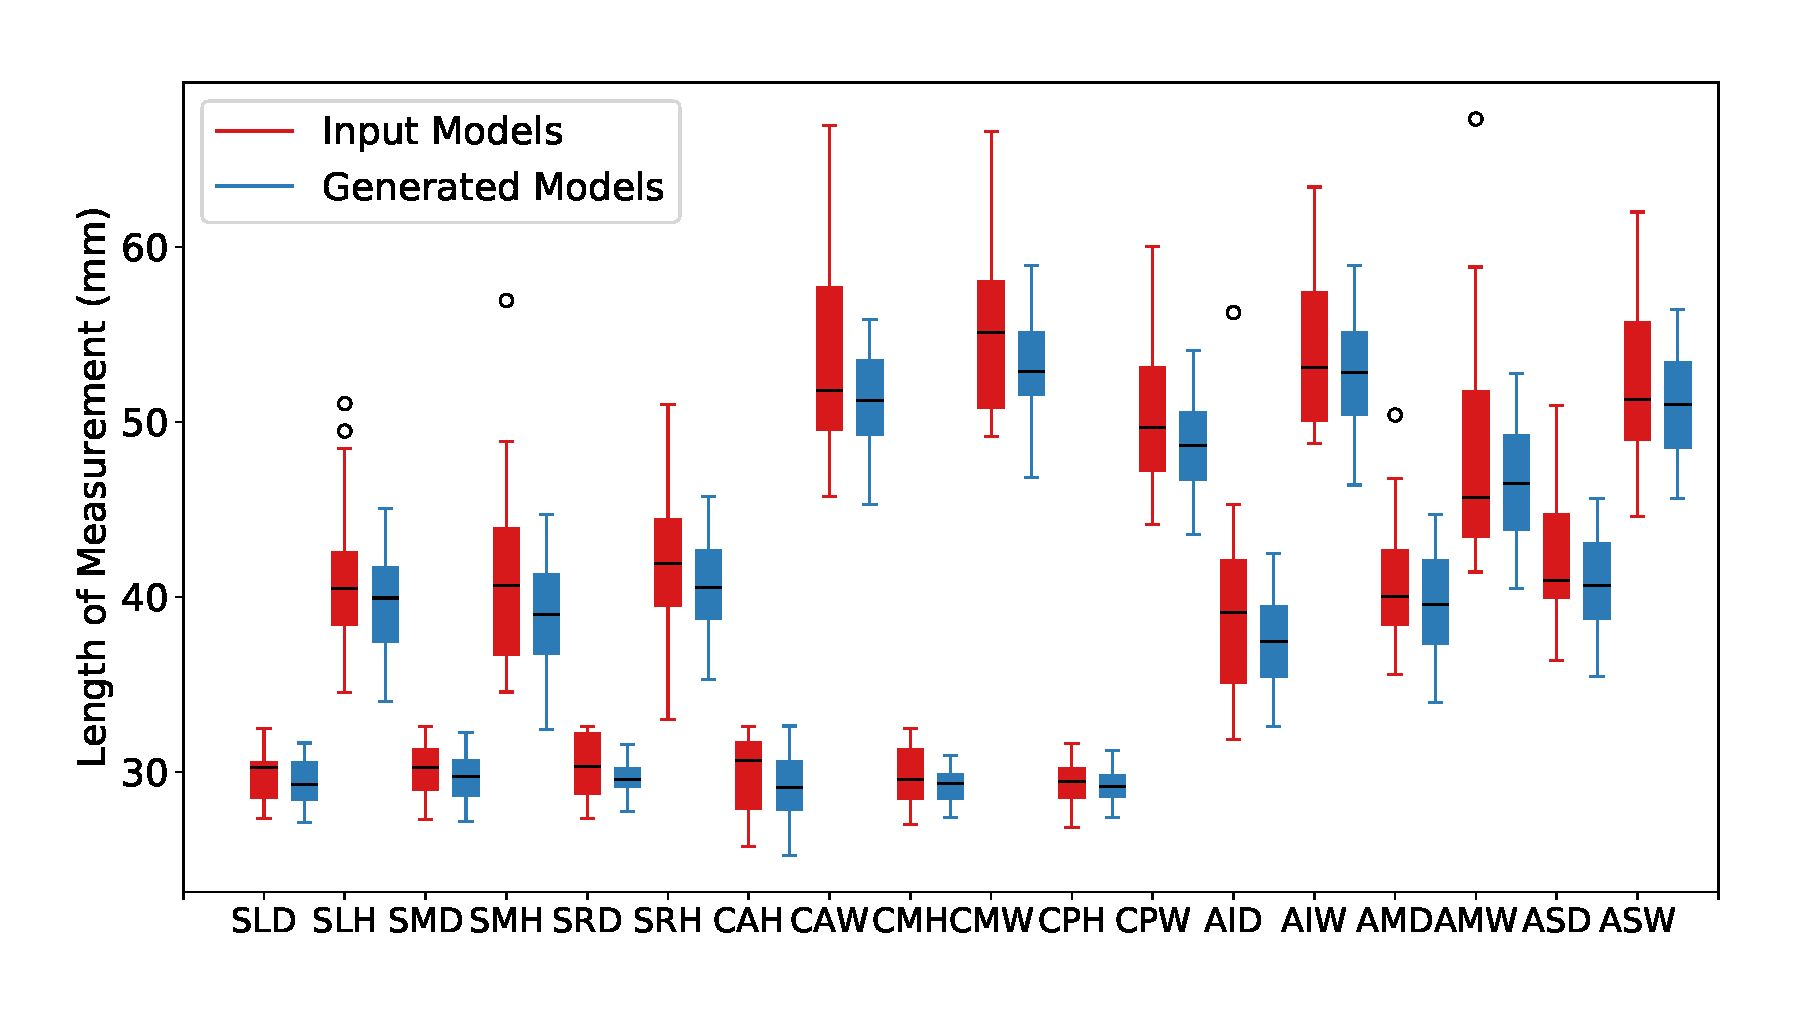
\includegraphics[width=\textwidth]{Chapters/Chapter_PCA_images/pca_cube.pdf}
	\caption{The variation in the 18 geometric measures of the input set models compared to the variation in the generated models for the first three principal components including all combinations of the +1, mean and -1 standard deviations.}
  \label{fig:pca_cube}
\end{figure}

\subsubsection{Material Property (Greyscale) Validation}


The variation seen in the histograms representing the greyscale differences between generated models and the input can be seen in \cref{fig:pc1_histo, fig;pc2_histo, fig:pc3_histo}, with the range of histograms from the input set shown as the grey range and the coloured lines showing the histogram for each of the generated models.
This normalised data shows a general agreement with the shape of the curves and relative quantities being very similar.
Deviations from the similarity are, for the most part, at the high and low greyscale values, where in general there are less voxels in this range for the generated models.
Comparing these results to a
\subsubsection{Resulting Stiffness Validation}


\subsection{Effect of Injected Cement Volume, Shape \& Position}



\subsection{Effect of Vertebral Variation on Augmentation}

\section{Discussion}
\label{pca_disc}

Validation

Modes of variation and how they represent the clinical problems (wedge shapes and fractures, small large, weak/stiff, etc.)

	
The response to small quantities of cement injected into the vertebrae is small. This is shown when comparing 20 \% fill volumes to 35 and 50 \% fill, where an increase in the stiffness is barely seen and only in the least dense vertebrae.
Attempts to understand the effect that the position of small volumes of cement (12 \% fill) has on the stiffness of the vertebrae shows sensible effects although a small percentage change to the stiffness of the vertebra compared to central positions of the cement volume.



Moving the cement volume in a lateral, left to right direction showed a reduction in stiffness when at the extremes of the vertebra, where the yielding interface of the cement volume encroached on the denser cortical shell defined by the greyscale background of the model.
The effect of the intermediate cement positions had a near symmetrical appearance - to be expected from the near symmetrical mean vertebra from the input set.

Inferior to superior movements of the cement showed a small change to the stiffness with a 2 \% increase to the superior of the vertebra, though a reduction when at the topmost point of the vertebra.
This can be explained by understanding the greyscale distribution of the model background or the material properties of the elements.
The element found in the centre of the vertebra are less dense and have a lower Young's modulus; when the cement was positioned in the centre and near superior, less of the low Young's modulus elements were exposed, resulting in an increased stiffness.

Moving the cement volume in a posterior to anterior direction showed a reduction in stiffness when at the extremes of the vertebra similarly to the lateral movements.
Away from the extremes, the stiffness rose to the anterior of the vertebra, where the bone is less dense in both natural specimens and these PCA generated models.
While this would suggest that vertebroplasty injections should always aim to the anterior of the vertebra (for purely stiffness increasing reasons, not just safety), the percentage change in stiffness from the least stiff - most posterior to the stiffest position is a mere 3 \%.
Given that the most stiff position still had a reduction of 13 \% compared to the non-augmented vertebrae, it suggests other factors may be more important and that the cement position, at least for small quantities of cement have little effect.

Compounding these results with the effect of cement position when varying the loading position... %TODO finish sentance

The effect of increasing the volume of the internal cement volume of the first three principal components affected the different models differently depending on what type of variation was found within that principal component.
As described previously small volumes of cement had little effect on the stiffness behaviour of the vertebral models, this extended to the 20 \% models where little to no increase in the stiffness was seen.
At 35 \% fill effects of the augmentation were seen, somewhat mirroring what was seen experimentally, where increases in the stiffness were only seen beyond approximately 35 \% fill.
The effect of increasing the cement from 20 through to 50 \% for the mean generated vertebra had the effect of increasing the stiffness near linearly %TODO CHECK
Larger increases in the stiffness were seen for the negative standard deviations away from the mean for PC1, where the main characteristic or mode of variation was the mean greyscale values and the negative standard deviations represented the least dense vertebra.
As expected these least dense vertebrae had a large increase in stiffness, increasing further with the increased volumes of cement.
Conversely, with the positive standard deviations away from the mean of PC1 which contained the densest vertebrae in the set, the increasing volume of cement reduced the stiffness of the vertebrae.
Again, this mirrored what was seen experimentally, where those specimens that had the highest bone volume fraction %TODO add where spines
had the smallest response to augmentation, with most showing a reduction in stiffness.
Computationally this reduction in stiffness is due to the replacement of dense material with high Young's moduli, to material with yielding properties and low Young's moduli (the interface region), despite the Young's modulus of the cement region itself being much higher than that of bone.
Experimentally, this reduction in stiffness could be due to the greater level of damage caused when inserting needles into the denser bone and other reasons described in Section \ref{Chapter_HT}. %TODO check I've done this and the ref is correct.

%TODO add papers - back up what i'm saying below.
Despite some studies suggesting that small quantities of cement (less that 20 \%) are enough to increase or restore the stiffness or properties of fractured vertebrae to that of the intact or natural vertebrae, the results presented here suggest otherwise.
Additionally, these studies lack any validation of experimental 

